\documentclass[a4paper, 12pt]{article}

\usepackage{other/lab_preamble}

\begin{document}
\LabTitle{2.2.5}{Определение вязкости жидкости по скорости истечения через капилляр}

\tableofcontents
\listoffigures \listoftables

\newpage

\textbf{Цель работы}:
\begin{enumerate}
  \item определение вязкости воды по измерению объёма жидкости, протекшей
        через капилляр

  \item определение вязкости других жидкостей путём сравнения скорости их перетекания
        со скоростью перетекания воды.
\end{enumerate}

\textbf{Приборы}:
\begin{enumerate}
  \item сосуд Мариотта

  \item капиллярная трубка

  \item набор мензурок

  \item секундомер

  \item микроскоп на стойке
\end{enumerate}

\section{Краткая Теория.}

Выделим в лминарном течении цилиндр \seefigref{fig:flux}.

\begin{figure}[H]
  \center
  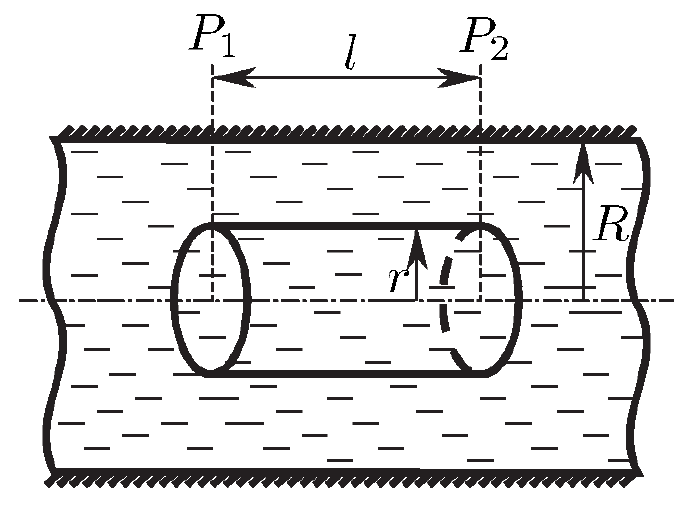
\includegraphics[scale=0.4]{data/pic1.png}
  \caption{Течение. \label{fig:flux}}
\end{figure}

\begin{equation}
  \tau = - \eta \deriv{v}{r}
\end{equation}
\begin{description}
  \item[$\tau$] - напряжение

  \item[$\eta$] - вязкость
\end{description}

\begin{equation}
  F_{\text{тр}}= S \eta \deriv{v}{r}
\end{equation}
\begin{description}
  \item[$F_{\text{тр}}$] - сила трения, действующая на поверхность цилиндра

  \item[S] - площадь поверхности цилиндра ($S = 2 \pi r l$)

  \item[$\deriv{v}{r}$] - градиент скорости
\end{description}

\begin{equation}
  (P_{1} - P_{2})\pi r^{2} + 2 \pi r l \eta \deriv{v}{r}= 0
\end{equation}

Интегрируя получим:
\begin{equation}
  v = \frac{P_{1} - P_{2}}{4\eta l}(R^{2} - r^{2})
\end{equation}

Формула Пуазейля для расхода жидкости Q через сечение трубки:
\begin{equation}
  Q \triangleq \frac{\Delta{V}}{\Delta{t}}= \pi \frac{P_{1} - P_{2}}{8 \eta l}R
  ^{4}
  % [Формула Пуазейля]
  % {Формула Пуазейля для расхода жидкости через сечение трубки}
  \label{eq:Poiseuille_formula}
\end{equation}

Число Рейнольдса:
\begin{equation}
  Re = \frac{v R \rho}{\eta}= \frac{2\frac{\rho v^{2}}{2}}{\eta \frac{v}{R}}\label{eq:Reynolds_number}
\end{equation}
\begin{description}
  \item[v] - характерная скорость течения

  \item[R] - радиус трубки (или "характерный размер")

  \item[$\rho$] - плотность газа или жидкости
\end{description}

Уравнение Бернулли:
\begin{equation}
  \frac{\rho v^{2}}{2}= P_{0} - P \label{eq:Bernoulli_eq}
\end{equation}

В гладких трубах круглого сечения переход от ламинарного течения к
турбулентному происходит при
\[
  Re \gtrapprox 1000
\]

Ламинарное движение жидкости при переходе из широкого сосуда в капилляр устанавливается
не сразу, а после того, как она пройдёт расстояние а:
\[
  a \approx 0,2 R Re
\]

\section{А. Измерение вязкости воды}
\subsection{Теория.}

\begin{figure}[H]
  \centering
  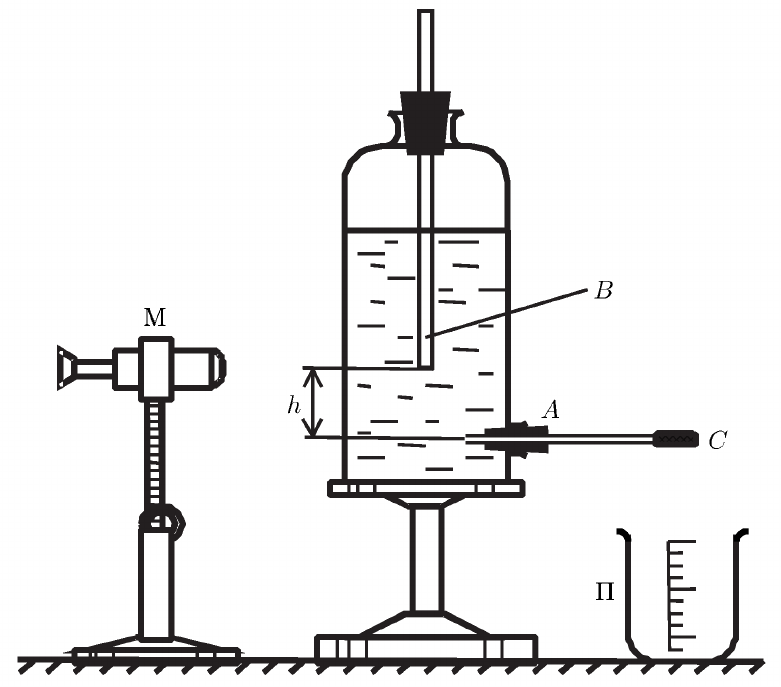
\includegraphics[scale=0.7]{data/a.png}
  \caption{Схема установки для определения вязкости воды.}
  \label{fig:vac}
\end{figure}

Установка для измерения вязкости воды изображена на \figref{fig:vac}. Вода заполняет
сосуд Мариотта и вытекает через капилляр, закрепленный в нижней части его
боковой стенки. Сосуд Мариотта позволяет поддерживать постоянный перепад давления
$P_{1} - P_{2}$ на капилляр, несмотря на то, что уровень жидкости при ее вытекании
понижается. Это достигается с помощью трубки В, открытой в атмосферу и проходящей
через пробку, герметично закрывающую сосуд. \par Величина перепада давления $P_{1}
  - P_{2}$ определяется высотой столба воды $h$ между осью капиллярной трубки А и
нижним концом вертикальной трубки В. Высота столба измеряется с помощью
микроскопа М, укрепленного на вертикально перемещающемся плунжере. Смещение
плунжера определяется по миллиметровой шкале. Объем вытекшей жидкости измеряется
мензуркой П. Время истечения определяется по секундомеру. Длина капиллярной трубки
указана на установке, диаметр - микроскопом.

\subsection{Ход работы}
\begin{enumerate}
  \item С помощь микроскопа определим радиус трубки:
        \[
          R = (0.8 \pm 0.1)\ \mm
        \]
        Зафиксируем длину капилляра:
        \[
          l = (13.7 \pm 0.1)\ \mm
        \]

  \item Закроем капиллярную трубку резиновой пробкой. Наполним сосуд Мариотта
        водой. \\ Снимим пробку и подождем, пока на нижнем конце трубки В не
        соскочит пузырек воздуха. \\ Это будет означать, что давление
        уравновесилось. \par Замечание: Не бойтесь, что вода потечет струей из капилляра,
        этого не произойдет, поток весьма слаб.

  \item Убедимся, что расход воды при одинаковой величине $h$ не зависит от
        уровня жидкости.\\ Для этого снимим пробку и замерим время, за которое вода
        наполнит мензурку на 20 - 25 мл. \\ (Данные утеряны)

  \item Перепад давлений $\Delta{P}$ между концами капилляра, не равен
        $\rho g h$, а содержит поправку $\Delta{h}$, обусловленную силами
        поверхностного натяжения. Чтобы её определить, будем опускть трубку В до
        тех пор, пока вода не перестанет вытекать из капилляра, это значит, что давление
        столба воды $\Delta{h}$ между осью капилляра и нижним торцом трубки В уравновесилось.
        $\Delta{P}= \rho g (h - \Delta{h})$.
        \[
          \Delta{h}\approx (10 \pm 0.1) \mm
        \]

  \item Измерим расход воды при нескольких значениях $h$. Результаты занесём в
        таблицу \ref{table:1}.
        \begin{table}[H]
          \center
          \begin{tabular}{|l|l|l|l|l|l|}
            \hline
            h, \mm & t, \sec & V, \ml & Q, \ml/\sec & Re  & a, \mm \\
            \hline
            30     & 310     & 10     & 0.03        & 1.8 & 0.3    \\
            47     & 353     & 20     & 0.06        & 3.0 & 0.5    \\
            64     & 280     & 20     & 0.07        & 3.3 & 0.5    \\
            70     & 204     & 20     & 0.10        & 5.5 & 0.9    \\
            \hline
          \end{tabular}
          \caption{Значения. 1 часть. \label{table:1}}
        \end{table}

  \item По формуле для числа Рейнольдса \ref{eq:Reynolds_number} удостоверимся,
        что в каждом из опытов в капилляре устанавливается ламинарное течение. По формуле
        $a = 0,2R \cdot Re$ оценим длину участка капилляра, по прохождении
        которого устанавливается ламинарное течение (см. таблицу \ref{table:1}).
        \par

        Т.к. $Re \ll 1000$ в каждом опыте, то течение можно считать ламинарным.

        \newpage

  \item Представим полученные результаты на графике $Q(h)$ \seefigref{fig:Q(h)}.

        \begin{figure}[H]
          \centering
          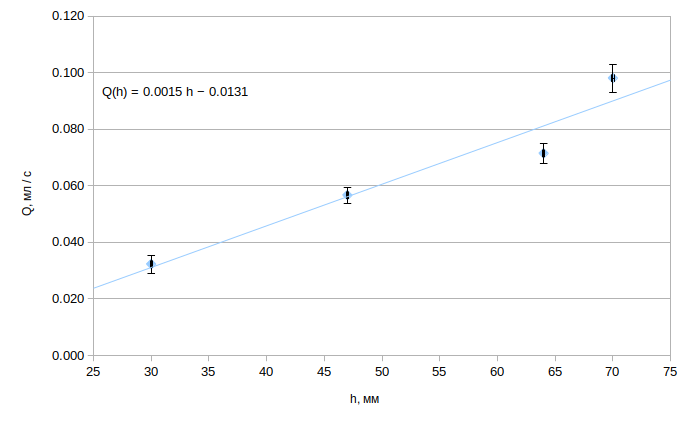
\includegraphics[scale=0.7]{data/Q(h).png}
          \caption{График зависимости расхода от высоты столба воды в сосуде}
          \label{fig:Q(h)}
        \end{figure}

        По формуле \ref{eq:Poiseuille_formula} видно, что зависимость должна быть
        линейной.

        \[
          Q = \frac{\pi R^{4} \rho g}{8 \eta l}(h - \Delta{h}) = \alpha h - \alpha
          \Delta{h}
        \]

        По МНК можно найти $\eta$ и $\Delta{h}$.

        \[
          \alpha = 0.015 \ \frac{\cm^{2}}{\sec}
        \]

        Оценим погрешность определения вязкости по формуле:
        \[
          \sigma_{\eta} = \eta \sqrt{4 \eps_{R}^{2} + \eps_{\alpha}^{2} + \eps_{l}^{2}}
          \approx 0,4 \ \mili \Puas
        \]

        Выражая $\eta$ через $\alpha$ получим:
        \[
          \eta = (7.8 \pm 0.4) \ \mili \Puas
        \]
        \label{water_viscosity}

        В действительности, при температуре $20\ \Celsius$ значение вязкости воды $\eta
          \approx 1\ \mili\Puas$. \\
\end{enumerate}

\section{Б. Измерение вязкости водного раствора глицерина\\ вискозиметром
  Оствальда}
\subsection{Теория.}

\begin{figure}[H]
  \centering
  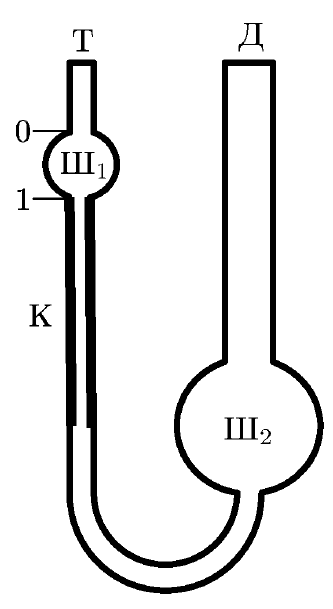
\includegraphics[scale=0.7]{data/b.png}
  \caption{Вискозиметр Оствальда.}
  \label{fig:Ostwald_viscometer}
\end{figure}

В части А вязкость жидкости определялась абсолюным методом, в этой части мы
будем использовать относительный метод. \\ Для измерений используется вискозиметр
Оствальда \seefigref{fig:Ostwald_viscometer}. \\ Считая известной вязкость одной
жидкости (воды - $\eta_{0}$), предлагается определить вязкость водного
раствора глицерина. \\

Вискозиметры Оствальда могут отличатся, но суть едина. \\ Мы хотим измерить
относительную разность во времени, за которое две жидкости проходят определенный
участок вискозиметра при одинаковых условиях. \\ У вискозиметра есть два
объема - Ш1 (который проходит жидкость) и Ш2 (в которой жидкость хранится). \\
На \figref{fig:Ostwald_viscometer} этот участок - [$0 \rightarrow 1$]. \\ Нас интересует
время, за которое столб жидкости на отметке 2 под действием сил тяжести
опустится до отметки 1. \\

\[
  \Delta{P}= P_{1} - P_{2} = \rho g h
\]

Пусть V - объем жидкости в области Ш1. Тогда h зависит от V (h(V)). Тогда формула
\eqref{eq:Poiseuille_formula} принимает вид:

\[
  -\deriv{V}{t}= \frac{\pi R^{4} \rho g h(V)}{8 \eta l}\implies
\]
\[
  \frac{\rho}{\eta}\ \Delta{t}= - \frac{8 l g}{\pi R^{4}}\int_{V_0}^{V_1}{\frac{\d{V}}{h(V)}}
  = const \quad (\text{не зависит от жидкости}) \implies
\]

\begin{equation}
  \frac{\rho_{1}}{\eta_{1}}\ t_{1} = \frac{\rho_{2}}{\eta_{2}}\ t_{2} \quad (\text{для
    двух жидкостей})
\end{equation}

Тогда зная $\eta_{0}, \rho_{0}, \rho$ и измерив время $t_{0}$, по времени прохождения
исследуемой жидкости t можно найти ее вязкость по формуле:
\begin{equation}
  \eta = \eta_{0} \frac{\rho}{\rho_{0}}\frac{t}{t_{0}}\label{eq:eta}
\end{equation}

\subsection{Ход работы}
\begin{enumerate}
  \item Промоем вискозиметр дистиллированной водой. Для этого заполним Ш2 и
        спринцовкой закачаем воду до отметки 2. Подождем, пока вода сольется.
        Промоем несколько раз.

  \item Определим время перетекания воды между метками. Измерения проведем 5-10
        раз. Результаты занесём в таблицу \ref{table:2}.

  \item Определим время перетекания 10-, 20-, 30-\% раствора глицерина. Для
        каждого раствора проведем 5-10 измерений. Результаты занесём в таблицу \ref{table:2}.

        \begin{table}[H]
          \center
          \begin{tabular}{|l|l|l|l|l|}
            \hline
                       &       & \multicolumn{2}{l}{Глицерин} &               \\
            \hline
                       & вода  & 10\%                         & 20\%  & 30\%  \\
            \hline
            1          & 13.18 & 18.84                        & 27.59 & 32.43 \\
            2          & 14.51 & 18.89                        & 26.87 & 32.69 \\
            3          & 14.87 & 18.78                        & 27.21 & 32.68 \\
            4          &       & 18.72                        & 26.9  & 33.1  \\
            5          &       & 18.78                        & 26.75 & 32.93 \\
            6          &       &                              &       & 32.78 \\
            \hline
            $\avrg{t}$ & 14.2  & 18.8                         & 27.1  & 32.8  \\
            \hline
            % \multicolumn{2}{l}{Дополнительные данные с другим вискозиметром Оствальда.} \\
            \hline
            1          &       & 7.87                         & 10.78 & 13.83 \\
            2          &       & 7.84                         & 11.08 & 13.79 \\
            3          &       & 7.97                         & 11.05 & 13.69 \\
            4          &       & 7.9                          & 10.9  & 13.7  \\
            5          &       & 7.95                         & 10.89 & 13.9  \\
            \hline
            $\avrg{t}$ &       & 7.9                          & 10.9  & 13.8  \\
            \hline
          \end{tabular}
          \caption{Значения времени перетекания жидкостей. \label{table:2}}
        \end{table}

        \paragraph{Замечание.}
        Таблица \ref{table:2} состоит из двух независимых подтаблиц. Первая - наши
        измерения, вторая - измерения нашего коллеги на другом вискометре.\\

  \item Определим плотность исследуемых растворов с помощью торсионных весов.
        \par Не проводили. Плотности возьмем из вне и приведем в таблице \ref{table:3}.

        \begin{table}[H]
          \center
          \begin{tabular}{|l|l|l|l|l|}
            \hline
                                       &      & \multicolumn{2}{l}{Глицерин} &             \\
            \hline
                                       & вода & 10\%                         & 20\% & 30\% \\
            \hline
            $\rho, \frac{\kg}{\m^{3}}$ & 1000 & 1022                         & 1047 & 1073 \\
            \hline
          \end{tabular}
          \caption{Плотности воды и глицерина. \label{table:3}}
        \end{table}

  \item Вычислим вязкость исследуемых растворов по формуле \eqref{eq:eta}. Оценим
        погрешность полученных результатов. \par Так как время измерялось
        секундомером, погрешность времени будет равна времени человеческой реакции,
        что примерно 0.3 секунды. \\ Значение и погрешность вязкости воды возьмем из
        предыдущей части. \\ Из \eqref{eq:eta} следует:
        \[
          \eps_{\eta} = \sqrt{\eps_{\eta_0}^{2} + \eps_{t_0}^{2} + \eps_{t}^{2} }
        \]

        Из прошлой части:
        \[
          \eta_{0} = (7.8 \pm 0.4) \ \mili\Puas, \quad \eps_{\eta} = 5.5\%
        \]

        Результаты приведены в таблице \ref{table:4}.

        \begin{table}[H]
          \center
          \begin{tabular}{|l|l|l|l|}
            \hline
                                         & \multicolumn{2}{l}{Глицерин} &             \\
            \hline
                                         & 10\%                         & 20\% & 30\% \\
            \hline
            $\eta,\ \mili\Puas$          & 10.6                         & 15.7 & 19.4 \\
            $\sigma_{\eta},\ \mili\Puas$ & 0.7                          & 1.0  & 1.2  \\
            $\eps_{\eta}$                & 6\%                          & 6\%  & 6\%  \\
            \hline
            \hline
            $\eta_{real},\ \mili\Puas$   & 1.31                         & 1.76 & 2.50 \\
            \hline
          \end{tabular}
          \caption{Значения времени перетекания жидкостей. \label{table:4}}
        \end{table}
\end{enumerate}

\section{Вывод.}
В ходе данной работы мы разными способами определили вязкости разных жидкостей:
абсолюным методом определили вязкость воды (см. \ref{water_viscosity}) и
относительным - вязкости растворов глицерина (см. таблицу \ref{table:4}).
\[
  \eta_{\text{воды}}= (7.8 \pm 0.4) \ \mili \Puas
\]
(что сильно отличается от истинного значения, к сожалению). \\
\end{document}